\documentclass[tikz,border=3pt]{standalone}
\usetikzlibrary{decorations.pathmorphing}
\begin{document}
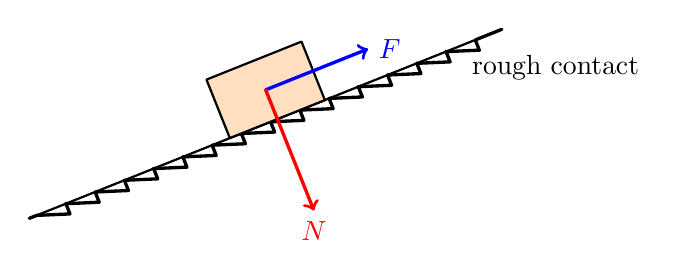
\begin{tikzpicture}[line cap=round,line join=round]
  \draw[thick] (0,0) -- (6,2.4);
  \draw[very thick,decorate,
    decoration={saw,segment length=4mm,amplitude=1.4mm,mirror,pre length=1mm,post length=1mm}]
    (0,0) -- (6,2.4);
  \begin{scope}[shift={(3.15,1.26)},rotate=21.8]
    \draw[fill=orange!25,thick] (-.65,0) rectangle (.65,.8);
    \draw[->,blue,very thick] (0,.4) -- (1.4,.4) node[right] {$F$};
    \draw[->,red,very thick] (0,.4) -- (0,-1.25) node[below] {$N$};
  \end{scope}
  \node[below right] at (5.5,2.2) {rough contact};
\end{tikzpicture}
\end{document}
